\chapter{Immersion Grating Design Considerations}

\section{Blaze angle and choice of R}
Blaze angle choice is an important early design consideration for Si immersion gratings.  There is a dichotomy in choice- R1.4 or anything else\footnote{The R-number is the tangent of the blaze angle, and is often used for specifying the blaze angle of echelles for example ranges R1-R10  correspond to $\delta= 45-84.2\deg$}.  The choice of R1.4 simplifies the substrate preparation process because R1.4 ($\delta=54.7$) is the natural blazing provided by the Si (111) crystal plane (see Figure \ref{fig:Rnum}).  One can simply cut Si pucks from conventionally prepared Si boules, with the cuts on parallel planes to the top (100) surface of the Si boule.  Different blaze angles require an additional sample preparation step of x-ray orienting and precision cutting substrates at finite angles from the conventional (100) Si boule surface.  For example, an R3 grating has $\delta=71.6 \deg=54.7\deg+16.9$.  So, cutting the Si boule at 16.9$\deg$ will yield R3 blazed facets.  The cutting plane is normal to the major flat plane.  The middle pane of Figure \ref{fig:IGdesignplot} shows the cutting angle as a function of the blaze angle, with the width of the line equal to the uncertainty of the cutting angle associated with finite etching into the (111) Si crystal plane.  


\begin{figure}[h!] 
\begin{center}
\ 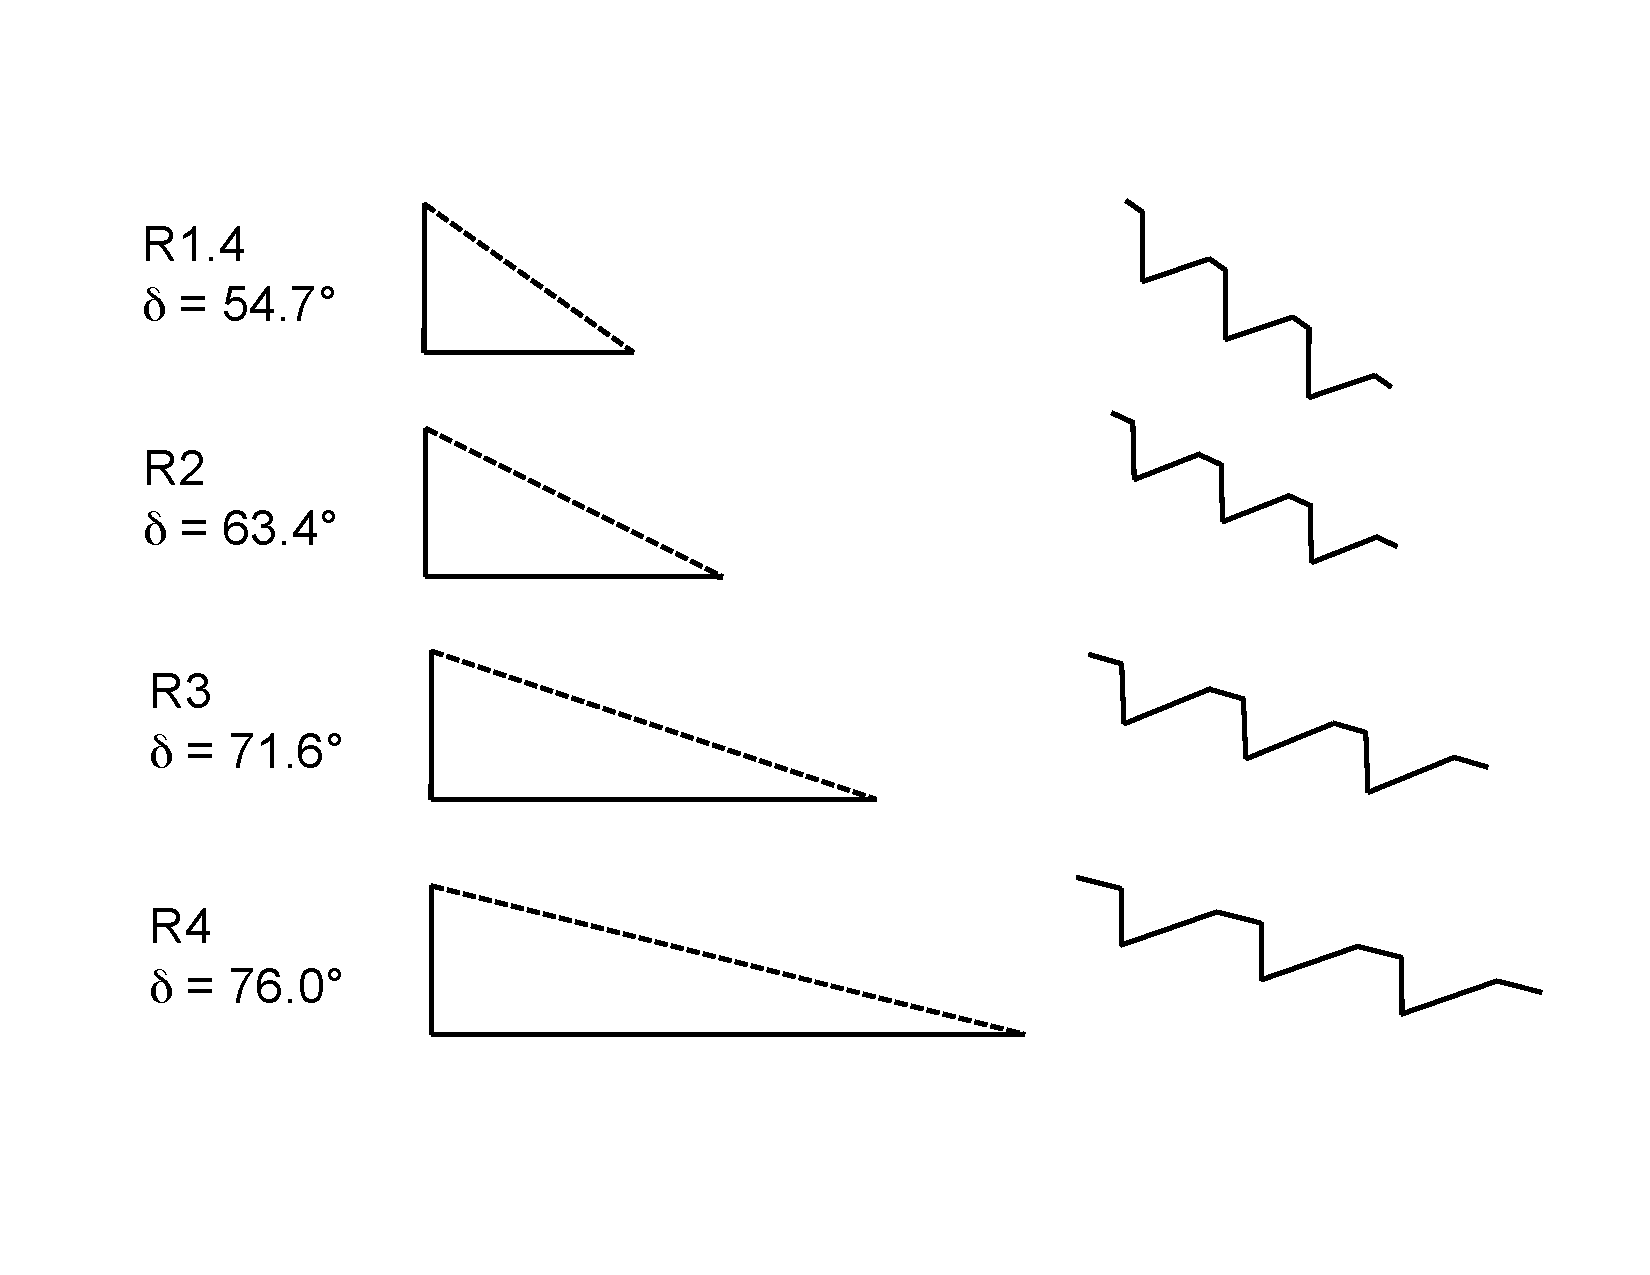
\psfig{file=chGratingDesign/Rnum,height=4.25in,width=5.5in}
\caption[Illustration of Si gratings of different blaze angles]{Illustration of Si gratings of different blaze angles, and the concomitant microscopic Si V-groove cross section.  The grooves are symmetric for R1.4, and increasingly asymmetric for larger blaze angles.  The apex angle of the cross section is 70.5$\deg$ in all cases; it is set by the Si crystal structure and is minutely increased by the finite anisotropic etch ratio.}
\label{fig:Rnum}
\end{center}
\end{figure}


\section{Groove top fill factor and geometric shadowing}
The groove top size has an allowable range.  The small size limit on the groove top is set by KOH under-etching, specifically the tops must be wide enough to hold up against the finite amount of under-etching.  Under-etching limits the groove top to a few percent of the groove width.  The large size limit for the groove top is set by geometric shadowing of the groove facets in a delivered device.  The geometric shadowing is illustrated schematically in Figure \ref{fig:groovetop}.  We derived the geometrical maximum groove top width above which the efficiency is degraded, described below.  We assumed for our derivation that light is incident normal to the groove facets, i.e. the Littrow configuration, which is a good assumption in immersion because of Snell's law.  The maximum allowable ratio of $t/\sigma$ is:

\begin{equation*}
t/\sigma < \frac{1}{1 + \frac{\tan(a)}{\tan(\delta)}}
\end{equation*}
Where $a$ is the Si Apex angle, and $\delta$ is the blaze angle.  For an R3 echelle we must have $t/\sigma < 0.51$.  For the LM module of iShell we elected to use a groove top $t=30 \; \mu$m, which is $t/\sigma=0.375$, so the groove tops will be safely shadowed in this device.  It makes sense that higher R-number gratings can tolerate larger groove tops, as can be surmised from the schematic Figure \ref{fig:groovetop} and the top pane of Figure \ref{fig:IGdesignplot}.


\begin{figure}[h!] 
\begin{center}
\ 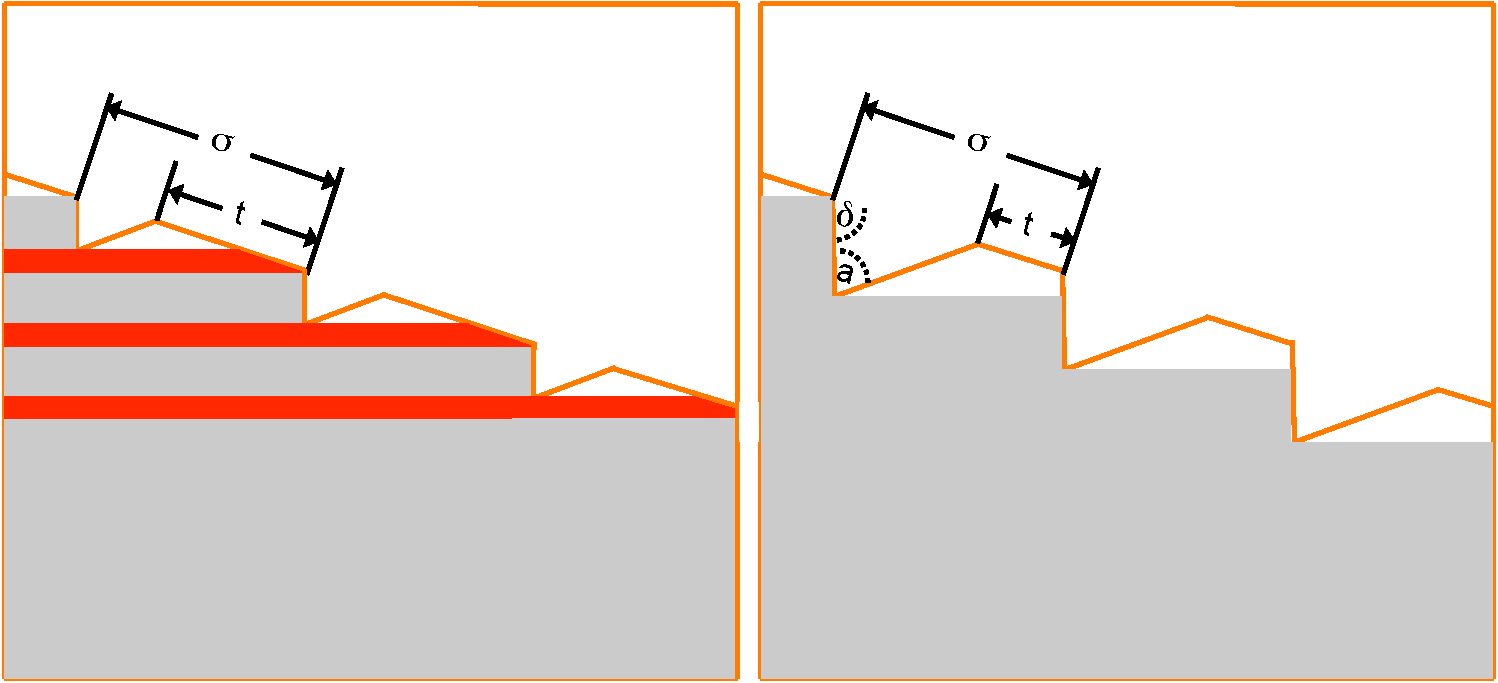
\psfig{file=chGratingDesign/gt_geom_blockage.pdf,height=3in,width=6.4in}
\caption[Schematic of groove top geometry]{Schematic of groove top geometry.  The cartoon gratings have the same blaze angle and period, but different groove top widths (fill factors).  There is a critical groove top width to period ratio below which the groove tops are completely shadowed and no geometric blockage occurs.  For an R3 grating as used in iSHELL, the critical fraction is $t/\sigma < 0.51$.  The delivered devices have $t/\sigma = 0.375$, which is similar to the schematic on the right side.}
\label{fig:groovetop}
\end{center}
\end{figure}

\begin{figure}[h!] 
\begin{center}
\ 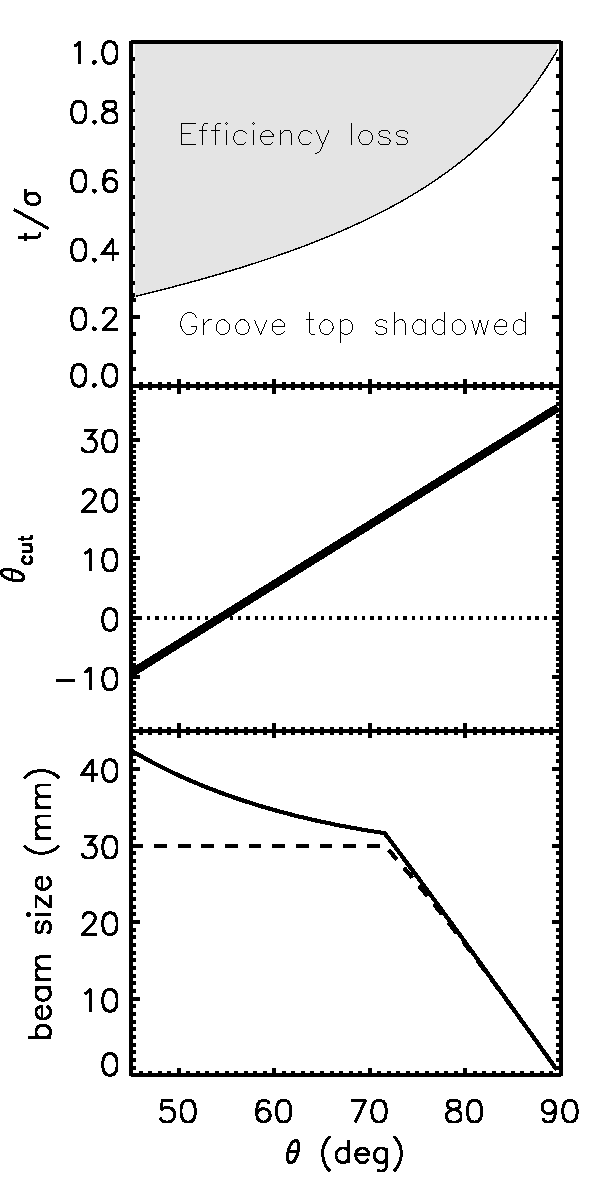
\psfig{file=chGratingDesign/IG_blaze_design.pdf,height=6.5in,width=3.25in}
\caption[Grating design considerations that depend on the choice of blaze angle]{Three paneled plot showing three grating design considerations that depend on the choice of blaze angle.  The top pane shows the range of groove top to grating period ratios that result in shadowed groove tops, or efficiency loss from exposed groove tops.  The middle pane shows the angle at which a Si boule must be cut to produce Si V groove facets at the given blaze angle.  The thickness of the line in the middle pane is equal to the range in cutting angle depending on the degree of anisotropic etching into the (111) Si crystal plane (and concomitant widening of the Si V-groove apex angle).  The width corresponds to $<0.8\deg$.  The bottom pane shows the maximum beam size possible on a 30 mm thick, 100 mm diameter Si substrate, as a function of blaze angle.  The solid line is the beam size, the dashed line is the substrate thickness as measured perpendicular to the grating surface.  These figures are all for Si immersion gratings in Littrow autocollimation.}
\label{fig:IGdesignplot}
\end{center}
\end{figure}

\subsection{Scarp face size in optical reflection measurements}
The proposed GMTNIRS grating LM module will require a larger beam size and a larger illuminated length than the IGRINS or iSHELL immersion gratings.  The strawman design requires an 8 inch substrate, which seems daunting given the challenges of immersion grating production on smaller 4 inch substrates.  Alternative designs employing an R4.5, rather than R3, grating are being considered.  High-R gratings have the limitation that the scarp facet length shrinks for larger blaze angles, until some threshold at which the scarp face is obscured.  The most important diagnostics for evaluating the performance of prototype immersion gratings require the scarp face to be visible.  

\begin{figure}[h!] 
\begin{center}
\ 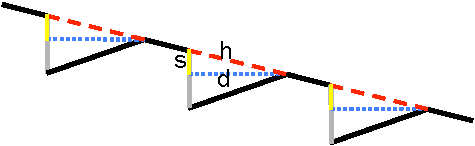
\psfig{file=chGratingDesign/scarp_reflect.pdf,height=2.0in,width=6.3in}
\caption[Scarp facet in reflection]{A diagram illustrating the lengths used to define the scarp face geometry when illuminated in back surface reflection.  The scarp face length $s$ is labelled and shown in the vertical short solid yellow line.  The blaze angle is the enclosed angle of line $s$ and $h$.  The hypotenuse of the right triangle is label $h$ in the long dashed red line.  The short blue dashed line is perpendicular to the scarp face and parallel to the incoming beam.  }
\label{fig:scarpface}
\end{center}
\end{figure}

Equipped with the geometrical definitions of \ref{fig:scarpface} we can determine $s$:
 \begin{eqnarray}
h=\sigma-t \nonumber \\
\cos{\delta}=s/h \nonumber \\
s=(\sigma-t)\cos{\delta}
 \end{eqnarray}

For an R4.5 grating, $\delta=77.5^\circ$, so the scarp facet $s$ is 20\% of the length $h=\sigma-t$.  There is no angle for which the scarp facet is completely shadowed, although it is true $s$ shrinks for large blaze angles.  Optical tests performed in reflection on higher blaze gratings will have a smaller scarp facet to probe, and the concomitant broad blaze envelope associated with convolving orders with the transform of narrow slit functions.  



